\section{Understanding the Landscape}
\label{sec:landscape}

Before explaining our attack, we need to better understand how Tor performs DNS
resolution.  We begin by investigating how common it is for adversaries
to be able to observe DNS request but \emph{not} subsequent TCP connections of
Tor users (Section~\ref{sec:as-exposure}).  We then seek to understand how
these results connect to the Tor network by determining the DNS resolvers used
by exit relays (Section~\ref{sec:mapping-resolvers}).

\subsection{Quantifying the additional AS exposure of DNS queries}
\label{sec:as-exposure}

Adversaries that can observe both DNS and subsequent TCP traffic (\eg, the ISP
of an exit relay) gain no benefit from seeing the client's DNS traffic,
since TCP traffic is sufficient to mount correlation
attacks~\cite{Murdoch2007a}.  In this work, we consider
adversaries that can observe traffic entering the Tor network and \emph{some}
DNS requests exiting the network---such as requests addressed to DNS
root servers---but {\em not} subsequent TCP traffic from exit relays.
We first determine the prevalence of these adversaries by measuring the
number of ASes that DNS queries traverse versus the
number of ASes subsequent web traffic traverses.

We quantify the {\em exposure} of DNS traffic versus TCP traffic as follows.  We
begin with Alexa's Top 1,000~\cite{alexatop1k}, a list of the 1,000 most popular
web sites as estimated by Alexa.  For each site, we conducted two
experiments.  First, we ran a TCP traceroute to the site, targeting port 80 to
mimic web traffic.  Second, we determined the DNS delegation path for the
website's DNS name using the {\tt dig} command's \texttt{+trace} feature.  The
delegation path of a domain name, say {\tt www.example.com}, is a list of
authoritative DNS servers, such as the authoritative server for {\tt .com}
pointing to the authoritative server of {\tt example.com}, which in turn points
to the authoritative server responsible for {\tt www.example.com}.  We also ran
UDP traceroutes to each server in the delegation path, targeting port 53 to
mimic DNS resolution.\footnote{The tool we developed for this purpose is
available online at \url{https://github.com/NullHypothesis/ddptr}.}
For both experiments, we then mapped all IP addresses in the traceroutes to AS
numbers~\cite{ipasn}, generating both a set of traversed ASes for DNS traceroutes
($\mathcal{D}$) and a set of traversed ASes for web traceroutes
($\mathcal{W}$).  Given these two sets for each of Alexa's Top
1,000, we compute the fraction of ASes that are \emph{only}
traversed for DNS traffic, but \emph{not} for web traffic ($\lambda$):

\begin{equation}
\label{equ:exposure}
\lambda \in [0, 1] =
\frac{|\mathcal{D} \setminus \mathcal{W}|}
     {|\mathcal{D} \cup \mathcal{W}|}.
\end{equation}
\noindent
The metric approaches 1 as the number of ASes that are only traversed for DNS
increases.  For example, if $\mathcal{D} = \{1,2,3\}$ and $\mathcal{W} =
\{2,3,4\}$, then $\lambda = \frac{|\{1\}|}{|\{1,2,3,4\}|} = \frac{1}{4} =
0.25$.  We determined $\lambda$ for each site in the Alexa Top 1,000.  We ran
the experiment on a French VPS in AS 16276, owned by OVH SAS.  We chose this AS
because, as of August 2016, it is the most popular AS by exit bandwidth, seeing
$10.98\%$ of exit traffic, closely followed by AS 12876 (owned by the French
Online S.A.S.) that sees $9.33\%$ of exit traffic.  The experiment resulted in
1,000~$\lambda$ values.  We repeated the experiment on a vantage point at our
institution, achieving similar results: while a two-sample Kolmogorov-Smirnov
test determined a statistically significant difference between both
distributions ($p \ll 0.01$), the medians (0.590 and 0.584) and standard
deviations (0.149 and 0.118) are similar.
% > ks.test(d1$exposure, d2$exposure)
%
%   Two-sample Kolmogorov-Smirnov test
%
% data:  d1$exposure and d2$exposure
% D = 0.1245, p-value = 6.218e-07
% alternative hypothesis: two-sided

Figure~\ref{fig:exposure} shows the empirical CDF of all 1,000~$\lambda$ values
that we calculated for Alexa's Top 1,000 sites.  In total, this experiment
traversed 350 unique ASes for DNS requests and 339 unique ASes for web requests.
The figure shows that for half of Alexa's Top 1,000 domains, DNS-only ASes
account for 60\% or more of all traversed ASes.  This result
only applies to exit relays that do their own DNS resolution; for relays that
use a third-party resolver, the ASes that are traversed between
the exit relay and its DNS resolver is the metric of interest.  We conclude that adversaries that are
unable to observe a Tor user's TCP connection still have many opportunities to
see a TCP connection's corresponding DNS request.  Such adversaries include (\emph{i}) popular open
DNS resolvers such as Google and OpenDNS, (\emph{ii}) DNS root servers, and
(\emph{iii}) network adversaries located on the path to the previous two
entities.

% d <- read.csv("top-1k-ddptr-2016-04-19-ovh.csv")
%> quantile(d$exposure)
%  0%   25%   50%   75%  100% 
%  0.000 0.500 0.600 0.667 0.909

\begin{figure}[t]
	\centering
	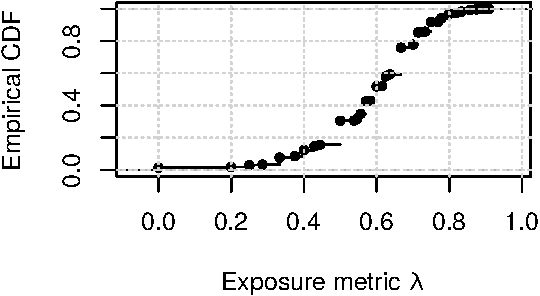
\includegraphics[width=0.75\linewidth]{figures/dns-exposure.pdf}
	\caption{Our AS exposure metric $\lambda$ for Alexa's Top 1,000 web sites.
	For half of all sites, 60\% of ASes or more are only traversed for DNS
	resolution, but not for subsequent web traffic.}
	\label{fig:exposure}
\end{figure}

\subsection{Determining how Tor exit relays resolve DNS queries}
\label{sec:mapping-resolvers}

Having shown that the Internet provides ample opportunity for
AS-level adversaries to snoop on DNS traffic from exit relays, we
now investigate how the exit relays in the Tor network resolve DNS
queries in practice. Before this study,
we only had anecdotal evidence (\eg, from OpenDNS-powered error
messages~\cite[\S~4.1]{Winter2014b}) that some exit relays would occasionally
show.

We identify the DNS resolver of all exit relays by using
exitmap~\cite{exitmap}, a scanner for Tor exit relays.  Exitmap automates
running a task such as fetching a webpage over all one thousand exit relays,
making it possible to see the Internet through the ``eyes'' of every single
exit relay.  Using exitmap, we resolve unique, relay-specific domains over
each exit relay, to a DNS server under our control.
Figure~\ref{fig:dnsenum} illustrates this experiment.  To improve reliability, we configured
exitmap to use two-hop circuits instead of the standard three-hop circuits.
The first hop was a guard relay under our control.  Over each exit relay, we
resolved a unique domain {\tt PREFIX.tor.domain.com}.  The prefix consisted of the
relay's unique 160-bit fingerprint, concatenated to a random 40-bit string
whose purpose is to prevent caching, so exit relays indeed resolve each query
instead of responding with a cached element.  We controlled the authoritative
DNS server of {\tt tor.domain.com}, so we could capture both the IP address and packet
content of every single query for {\tt tor.domain.com}.

\begin{figure}[t]
	\centering
	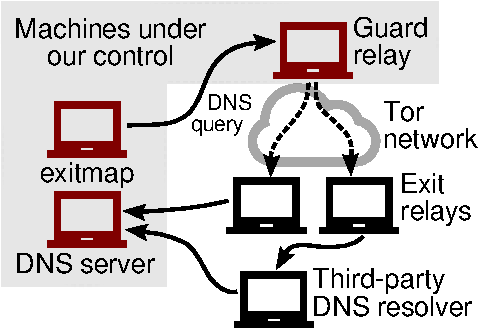
\includegraphics[width=0.6\linewidth]{figures/resolver-identification.pdf}
	\caption{Our method to identify the DNS resolvers of exit relays.  Over
	each exit relay, we resolve relay-specific domain names that are under our
	control.  Inspecting our DNS server logs, we can then identify the IP
	address of all exit relay resolvers.}
	\label{fig:dnsenum}
\end{figure}

An exit relay can either run its own resolver, as shown in the left exit relay in
Figure~\ref{fig:dnsenum}; or rely on a third-party resolver, such as the one
provided by its ISP, as shown in the right exit relay in Figure~\ref{fig:dnsenum}.  If
an exit relay runs its own resolver, we expect to receive a DNS request from
the exit relay's IP address, but if an exit relay uses a third-party resolver,
we expect to receive a request from an unrelated IP address.  Having encoded
relay-specific fingerprints in the query names, we are able to map queries to
exit relays in such cases.  We ran this experiment from September 2015 to May
2016, at least once a day.  Once we started to analyze our data, we identified
the following two challenges:

\begin{itemize}
\item {\em DNS proxies:}
We found that several exit relays used DNS
proxies---machines that passed on DNS requests to an actual resolver
instead of resolving it themselves.  Google's server {\tt 8.8.8.8} is a popular
example of a DNS proxy;
several dozen machines perform resolution in the
background~\cite{google-proxies}.  DNS proxies do
not interfere with our measurements, so we ignored them.

\item {\em Multiple DNS resolvers:}
On Linux systems, DNS resolution is controlled by the file
\texttt{/etc/resolv.conf}.  It contains a list of up to three DNS resolvers
that are queried in order.  If the primary resolver does not respond within a
time limit, the system falls back to the second, and finally the third
resolver.  Our data suggests that several exit relays used
different resolvers in subsequent exitmap scans---one relay, for example, used
both Google's DNS resolver and one provided by its ISP.  For our visualization,
we only consider the first resolver we observed for an exit relay, which might
not be the primary resolver.
\end{itemize}
\noindent
Figure~\ref{fig:exit-resolvers} illustrates the fraction of DNS requests that
four of the most popular organizations could observe.  Google averages at 33\%,
but at times saw more than 40\% of all DNS requests exiting the Tor network---an
alarming number for a single organization.  Second to Google is ``Local''---exit
relays that run their own resolver, averaging at 12\%.  Next is OVH, which used
to be as popular as local resolvers, but slowly lost its share over time.  Note
that in contrast to Google, OVH does not run a public DNS server; the company's
resolvers are only accessible to its customers.  Finally, there is OpenDNS,
which also runs public DNS resolvers.  OpenDNS saw occasional spikes in
popularity but always remained in the single digits.  Apart from the illustrated
top resolver setups, the distribution has a long tail, presumably consisting of
many ISP resolvers.

\begin{figure*}[t]
	\centering
	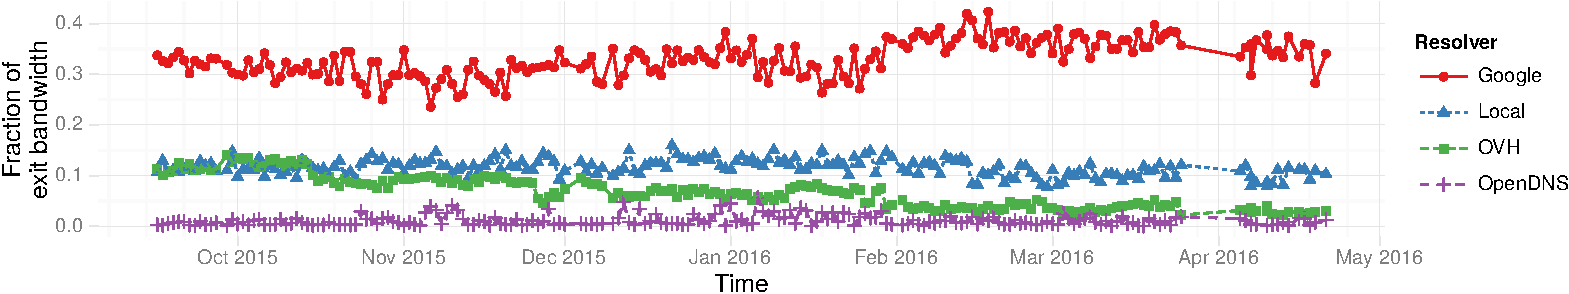
\includegraphics[width=\linewidth]{figures/asn-bw-frac.pdf}
	\caption{The popularity of some of the most popular DNS resolvers of exit
		relays over time.  The $y$ axis depicts the fraction of exit bandwidth
		that the respective resolver is responsible for.  Google's DNS resolver
		is by far the most popular, at times serving more than 40\% of all DNS
		requests coming out of the Tor network.  Google is followed by local
		resolvers, which average at around 12\%.  Once serving a fair amount of
		traffic, OVH dropped in popularity, and is now close to OpenDNS, an
		organization that runs an open resolver.}
	\label{fig:exit-resolvers}
\end{figure*}

% The following section takes up too much space, so it's commented out for now.
% We should include it in an extended version of our work, though.

\iffalse
\subsection{Inferring resolver configuration}
\label{sec:mapping-configuration}

In addition to identifying an exit relay's DNS resolver, our measurement
techniques can ascertain aspects of the of how an exit relay's local
resolver are configured.  It is important to identify broken resolvers
because they jeopardize the anonymity of Tor users.  Resolvers with poor
or broken configuration pose a security risk to Tor users as attackers
could poison or enumerate their cache, allowing them to redirect users
or profile them. Below, we discuss certain aspects of Tor's DNS resolver
configurations that we can infer with our measurements.

\paragraph{Random source ports}
To impede cache poisoning attacks, DNS resolvers should use random
source ports instead of always using UDP port 53.  Our measurements can
determine whether a given resolver randomizes its source ports.  We
classify a resolver as ``uses randomization'' if the source port does
not equal 53.  This method causes a small number of false positives
because a randomizing resolver could use port 53 simply by chance.  The
probability of that happening is only $\frac{1}{65535}$.

We found 135 DNS resolvers that did not use random source ports.  These
resolvers were located in the networks of Vodafone, Germany (95\%), MTNL, India
(4\%), and Cogent, U.S. (1\%).

\paragraph{0x20 encoding}
Resolvers can further reduce the chance of cache poisoning by employing
{\tt 0x20} encoding (\ie, randomizing the capitalization of domain
names).  For example, to resolve {\tt foo.com}, a resolver would send a
request for {\tt fOo.CoM}.  If the DNS response does not reflect the
randomly chosen capitalization, the resolver considers unauthentic.  We
classify a resolver as ``uses {\tt 0x20}'' if it has at least one
lowercase and one uppercase character.  Again, there is a chance of
false positives, which depends on the domain name length.  A {\tt
  0x20}-encoded domain name of $n$ characters (excluding periods) can be
all-uppercase or all-lowercase with probability $2 \cdot 0.5^n$.

We found 427 DNS resolvers that did not use 0x20 encoding for at least one
query.  The top five resolvers were located in the networks of Google, U.S.
(38\%), AT\&T, U.S. (22\%), Deutsche Telekom, Germany (7\%), Yandex, Russia
(7\%), OpenDNS, U.S. (4\%).

\paragraph{DNSSEC validation}
We can verify whether a resolver is validating DNSSEC-signed records by resolving a
domain whose signature is deliberately malformed; 
{\tt dnssec-failed.org} provides such a service.  A validating resolver
would not return an {\tt A} record while
a non-validating resolver would.  Therefore, we send an {\tt A} query {\tt dnssec-failed.org} via
all exit relays and check whether we receive an response
\fi
